\section{Planning}\label{sec:Planning_arkitektur}

Planningwidget skal benyttes til planlægning af lige hvad man som bruger, har brugt for at planlægge. Derfor er det også væsentlig, at en planning kan konfigureres til brugerens behov. En planningwidget er tilknyttet en gruppe, men samtidig er den ikke nødvendigvis til alle gruppens medlemmer. Derfor skal der være muligt at tilføje/fjerne brugere til/fra en planning. Ud over disse overvejelser, så er der nogle US, som skal kunne gennemføres. Arkitekturen vil tage grundlag i disse US. Detaljerede US kan findes i bilag \cite{KravspecUserStoriesPlanning}.

\subsection{Data view}

\noindent Ud fra US tilknyttet planning, er nogle entities bestemt: Planning, Shift, UsersInPlanning, UsersShift og UserSwapShiftNotify. Disse skal udgøre tabellerne i databasen for planning. Hertil skal passende relationer bestemmes, så ledes, at en planning kan indeholde flere shifts, samt flere UsersInPlanning. UsersShift skal indeholde composite keys, bestående af UsersInPlanning id'er og Shift Id'er. 
\\ \\ 
UserSwapShiftNotify skal indeholde notifikationer for bytning af vagter mellem to brugere, hvortil passende attributer er blevet tilknyttet. Ud fra disse overvejelser er et ER-digram udarbejdet, som kan ses nedenfor på figur \ref{fig:ark_planning_data_dbview}.

\begin{figure}[H]
  \includegraphics[width=\linewidth]{09_Arkitektur/Planning/pictures/DB_Planning.jpg}
  \caption{ER Diagram for plannings til Database strukturen. OneToMany relationer fra planning til både Shift og UsersInPlanning. OneToMany fra Shift til UsersShift, samt fra UsersInPlanning til UsersShift. Samme relation benyttet til UserSwapShiftNotify.}
  \label{fig:ark_planning_data_dbview}
\end{figure}

\noindent Ud fra ER-diagrammet, er det muligt at designe modeller til planning.
\subsection{Logical view}\label{ssec:planlaegning:logicalview}
Dette afsnit skal forklare applikationslogikken for plannings i webapplikationen.
\\ \\
Bussiness logikken vil blive lagt i en controller, for at overholde MVC strukturen. Dertil vil PlanningControlleren komme til at stå for at håndtere brugers anmodninger og render views med modeldata. Til udarbejdelsen af arkitekturen for PlanningControlleren er der lagt vægt på US's, hvor der er arbejdet agilt med dokumentationen samt implementeringen. Dertil er ikke alle US implementeret endnu, men vil blive i fremtidige iterationer. \\

\noindent Ud fra arkitekturen beskrevet i bilag \cite{ArkitekturPlanning}, så er et klassediagram udarbejdet, som der kan tages udgangspunkt i til design og implementeringen. Klassediagrmmet ses nedenfor på figur \ref{fig:ark_planning_logic_classdiagram}.

\begin{figure}[H]
  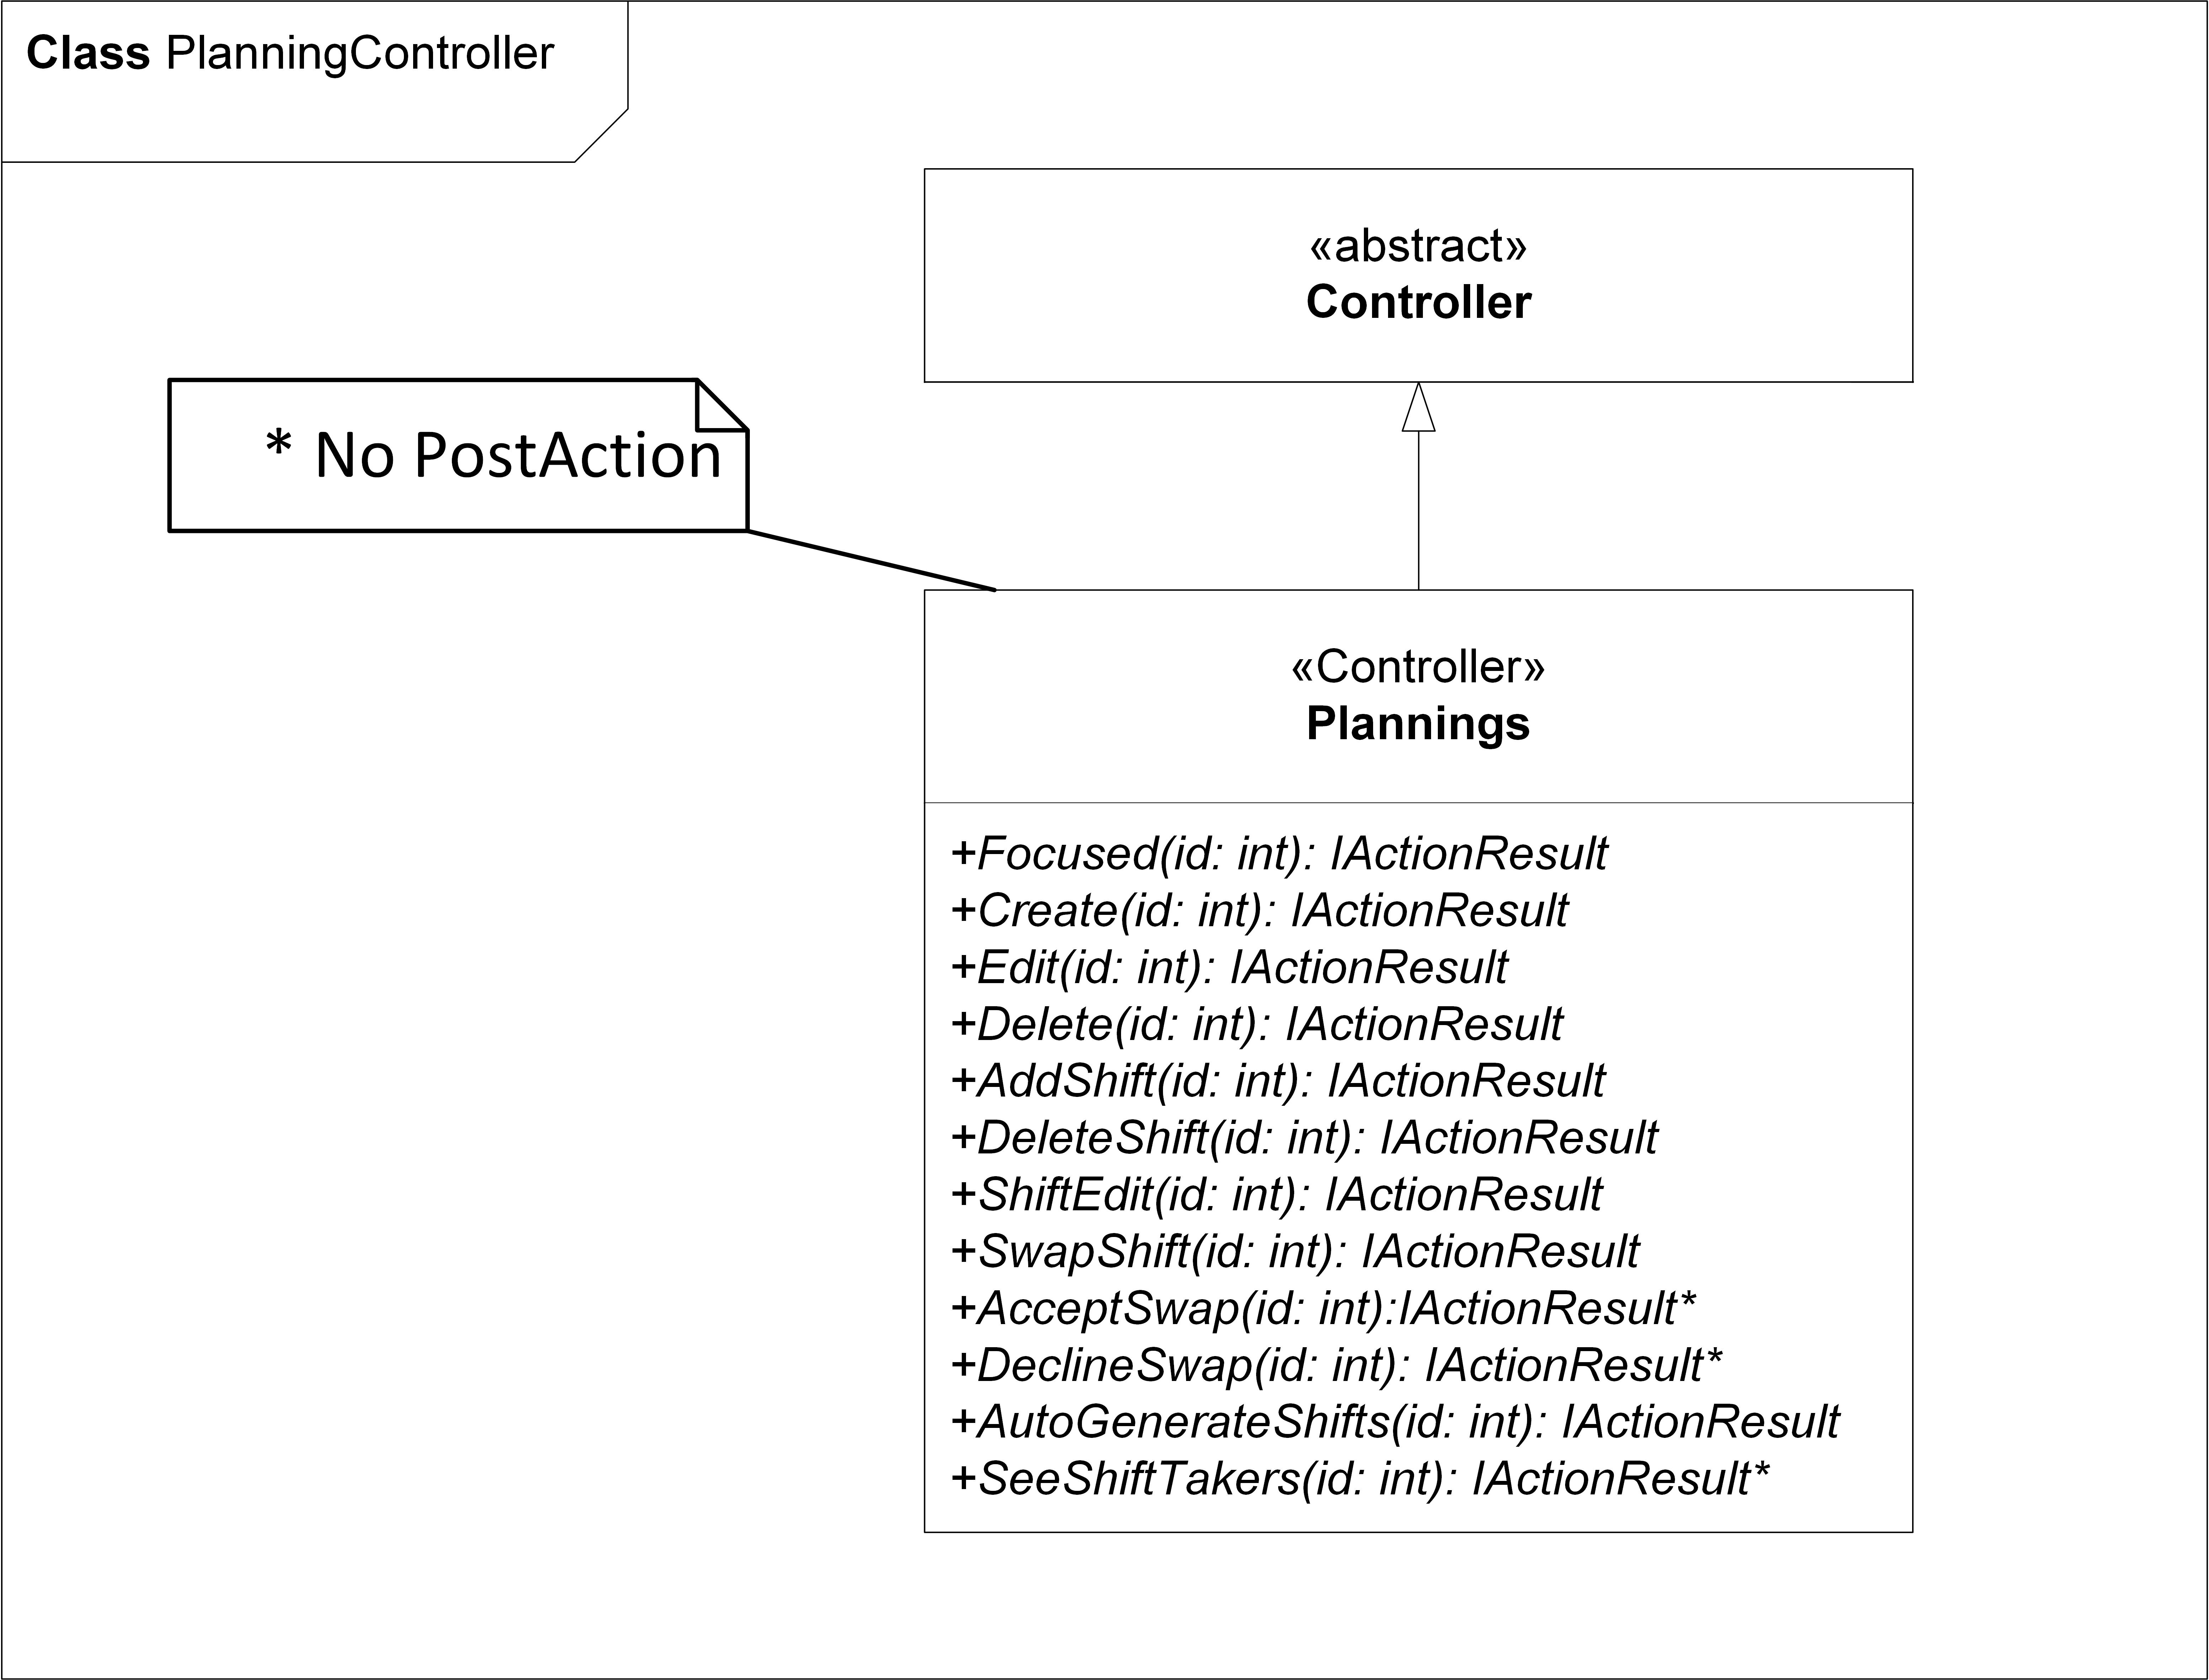
\includegraphics[scale=0.8]{09_Arkitektur/Planning/pictures/CD_Planning.jpg}
  \centering
  \caption{Klassediagram for planningController med de nødvendige metoder til at gennemføre de valgte US}
  \label{fig:ark_planning_logic_classdiagram}
\end{figure}


